\section{ニューラルネットワーク}
前章ではパーセプトロンについて学びましたが,パーセプトロンについては良いニュースと悪いニュースがありました.良いニュースとは,パーセプトロンの複雑な関数であっても,それを表現できるだけの可能性を秘めているということです.悪いニュースは,重みを設定する作業は,今のところ人の手で行われているということです.

ニューラルネットワークは,先の悪いニュースを解決するためにあります.具体的に言うと,適切な重みパラメータをデータから自動で学習できるというのがニューラルネットワークの重要な性質のひとつです.本章では,ニューラルネットワークの概要を説明し,ニューラルネットワークが識別を行う際の処理に焦点を当てます.そして,次章にて,データから重みパラメータを学習する方法を学びます.
\subsection{パーセプトロンからニューラルネットワークへ}
ニューラルネットワークは,前章で説明したパーセプトロンと共通する点が多くあります.
\subsubsection{ニューラルネットワークの例}
ニューラルネットワークを図で表すと,\fref{fig:3_NeuralNetwork}のようになります.ここで,一番左の列を\textbf{入力層},一番右の列を\textbf{出力層},中間の列を\textbf{中間層}(隠れ層)と呼びます.本書では,入力層から出力層ンい向かって,順に第0層,第1層,第2層と呼ぶことにします.

\begin{figure}[h]
  \vspace{0mm}
  \begin{center}
    \hspace{0mm}
    \centering
    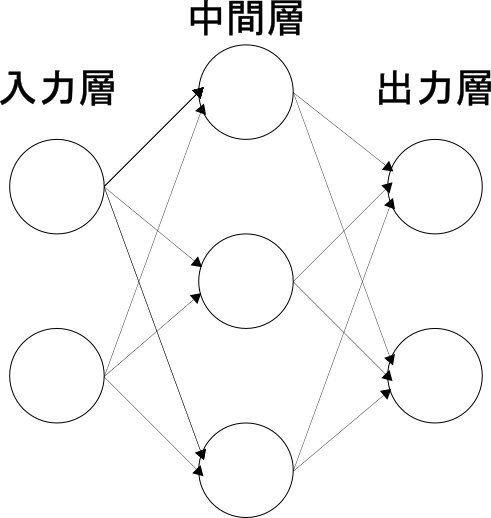
\includegraphics[width=30mm]{Ch3/NeuralNetwork.png} \
    \vspace{0mm}
    \caption{ニューラルネットワークの例}
    \label{fig:3_NeuralNetwork}
  \end{center}
\end{figure}

\subsubsection{パーセプトロンの復習}

\begin{figure}[h]
  \vspace{0mm}
  \begin{center}
    \hspace{0mm}
    \centering
    \includegraphics[width=30mm]{Ch2/peceptron2.png} \
    \vspace{0mm}
    \caption{パーセプトロンの復習}
    \label{fig:3_peceptron2}
  \end{center}
\end{figure}

\fref{fig:3_peceptron2}を数式で表すと\eref{eq:3_peceptron}のようになります.

\begin{equation}
    \label{eq:3_peceptron}
    y = \left\{
\begin{array}{ll}
0 & (b + \omega_1 x_1 + \omega_2 x_2 \le 0)\\
1 & (b + \omega_1 x_1 + \omega_2 x_2 > 0)
\end{array}
    \right.
\end{equation}

$b$を明示したものを\fref{fig:3_vias}に示す.\eref{eq:3_peceptron}をよりシンプルな形に書き換える.

\begin{figure}[h]
  \vspace{0mm}
  \begin{center}
    \hspace{0mm}
    \centering
    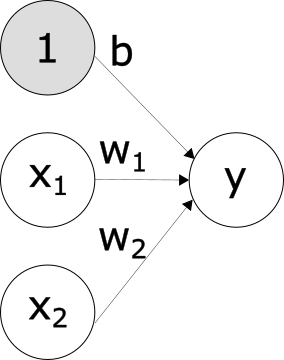
\includegraphics[width=30mm]{Ch3/vias.png} \
    \vspace{0mm}
    \caption{バイアスを明示的に示す}
    \label{fig:3_vias}
  \end{center}
\end{figure}




\eref{eq:3_peceptron_simple}は,入力信号の総和が$h(x)$という関数によって変換され,その変換された値が出力$y$になるということを表しています.そして,\eref{eq:3_step_function}で表された$h(x)$関数は,入力が0を超えたら1を返し,そうでなければ1を返します.そのため,\eref{eq:3_peceptron}と\eref{eq:3_peceptron_simple},\eref{eq:3_step_function}は同じことを行っているのです.

\subsubsection{活性化関数の登場}
**..

\begin{equation}
    \label{eq:3_peceptron_simple2}
a=b+\omega_1 x_1 + \omega_2 x_2
\end{equation}

\begin{equation}
    \label{eq:3_step_function2}
y=h(a)
\end{equation}

\eref{eq:3_peceptron_simple2}では,重み付き入力信号とバイアスの総和を計算し,それを$a$とします.\eref{eq:3_step_function2}では,$a$が$h(x)$で変換され$y$が出力される,という流れになります.

それでは続いて活性化関数について詳しく見ていくことにします.この活性化関数が,パーセプトロンからニューラルネットワークへ進むための懸け橋になります.\footnote{「パーセプトロン」という言葉がさすアルゴリズムは,本書では厳密な統一がされずに使われています.一般的に,「単純パーセプトロン」といえば,それは単層のネットワークで,活性化関数にステップ関数を使用したモデルを指します.「多層パーセプトロン」というと,それはニューラルネットワーク-多層で,シグモイド関数などの滑らかな活性化関数を使用するネットワーク-を指すのが一般的です.
}


\subsection{活性化関数}
「パーセプトロンでは、活性化関数にステップ関数を利用している」ということができる。つまり、活性化関数の候補としてたくさんある関数の中で、パーセプトロンは「ステップ関数」を採用しているのです。活性化関数にステップ関数以外の関数を採用することで、ニューラルネットワークの世界へと進むことができるのです!

\subsubsection{シグモイド関数}
ニューラルネットワークでよく用いられる活性化関数の一つは、\eref{eq:3_sigmoid}で表されるシグモイド関数です.

\begin{equation}
    \label{eq:3_sigmoid}
    h(x) = \frac{1}{1 + \exp(-x)}
\end{equation}

前章で見たパーセプトロンとこれから見ていくニューラルネットワークの主な違いは、この活性化関数だけなのです。

\subsubsection{ステップ関数の実装}
\ShowPython{THstep.py}
\begin{figure}[H]
  \vspace{0mm}
  \begin{center}
    \hspace{0mm}
    \centering
    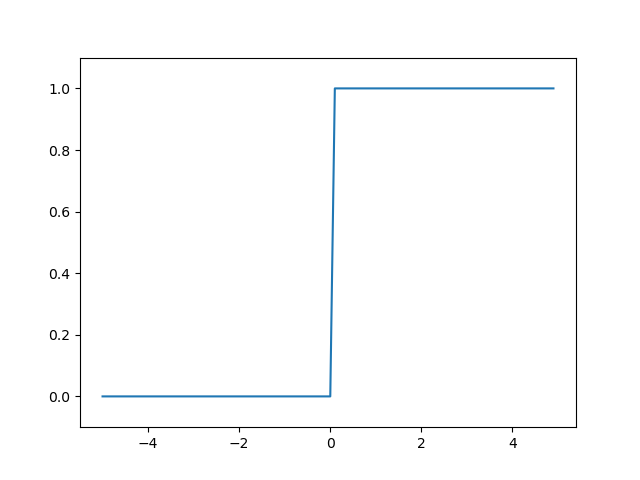
\includegraphics[width=40mm]{Ch3/step.png} \
    \vspace{0mm}
    \caption{ステップ関数のグラフ}
    \label{fig:3_step}
  \end{center}
\end{figure}

\subsubsection{シグモイド関数の実装}
\ShowPython{THsigmoid.py}
\begin{figure}[h]
  \vspace{0mm}
  \begin{center}
    \hspace{0mm}
    \centering
    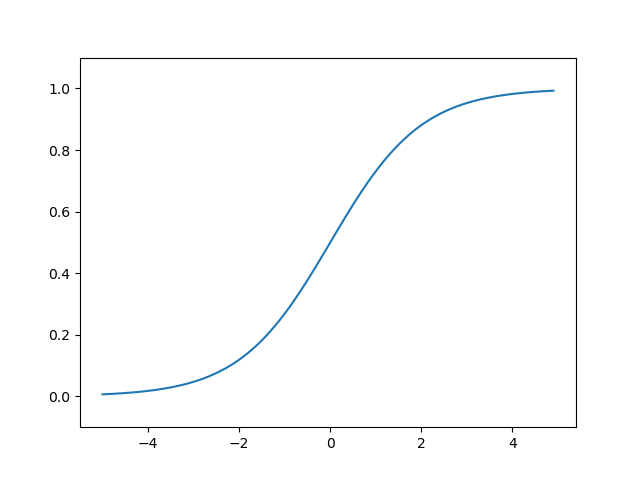
\includegraphics[width=40mm]{Ch3/sigmoid.png} \
    \vspace{0mm}
    \caption{シグモイド関数のグラフ}
    \label{fig:3_sigmoid}
  \end{center}
\end{figure}

\subsubsection{シグモイド関数とステップ関数の比較}
\ShowPython{THstepsigmoid.py}
\begin{figure}[H]
  \vspace{0mm}
  \begin{center}
    \hspace{0mm}
    \centering
    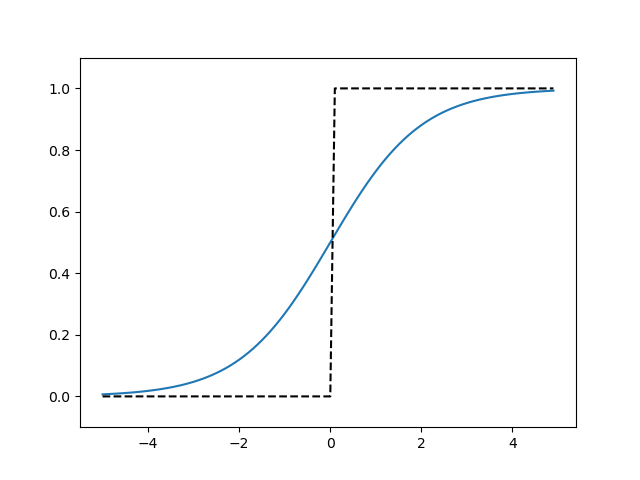
\includegraphics[width=50mm]{Ch3/SigmoidStep.png} \
    \vspace{0mm}
    \caption{ステップ関数とシグモイド関数(破線はステップ関数)}
    \label{fig:3_SigmoidStep}
  \end{center}
\end{figure}

両者とも、入力信号が重要な情報であれば大きな値を出力し、入力信号が重要でなければ小さな値を出力するのです。そして、どんなに入力信号の値が小さくても、またどんなに入力信号の値が大きくても、出力信号の値を0から1の間に押し込めるのも両者の共通点です。

\subsubsection{非線形関数}

\subsubsection{ReLu関数}
これまでに活性化関数としてステップ関数とシグモイド関数を紹介しました。シグモイド関数は、ニューラルネットワークの歴史において、古くから利用されてきました。しかし、最近では\textbf{ReLU関数}(Rectified Linear Unit)という関数が主に用いられます(\fref{fig:3_relu}参照)。

\ShowPython{THrelu.py}
\begin{figure}[h]
  \vspace{0mm}
  \begin{center}
    \hspace{0mm}
    \centering
    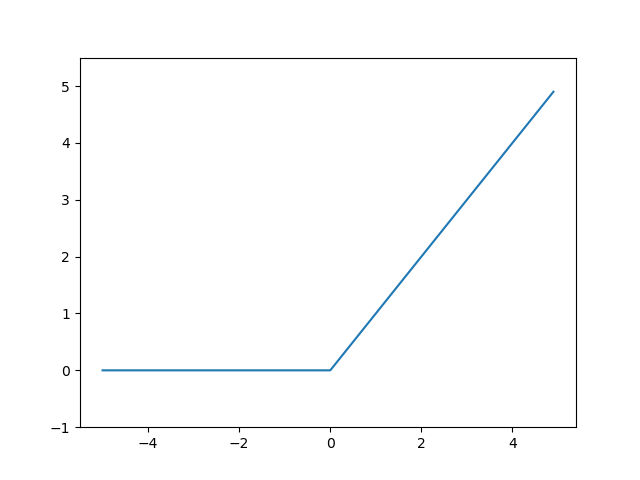
\includegraphics[width=50mm]{Ch3/relu.png} \
    \vspace{0mm}
    \caption{ReLU関数}
    \label{fig:3_relu}
  \end{center}
\end{figure}

ReLU関数を数式で表すと、\eref{eq:3_relu}のようになります。

\begin{equation}
    \label{eq:3_relu}
    h(x) = \left\{
\begin{array}{ll}
x & (x > 0)\\
0 & (x \le 0)
\end{array}
    \right.
\end{equation}

グラフや数式の通り、ReLU関数はとてもシンプルな関数です。そのため、実装もとても容易です。

さて、本章の残りでは、活性化関数にシグモイド関数を使用していきますが、本書の後半では主にReLU関数を使用していきます。

\subsection{多次元配列の計算}
ここではNumpyによる多次元配列の計算について説明し、その後にニューラルネットワークの実装を行っていきます。
\subsubsection{多次元配列}
\subsubsection{行列の積}
\subsubsection{ニューラルネットワークの行列の積}

